%!TEX program = xelatex
% not lualatex because of a pgf bug: https://sourceforge.net/p/pgf/bugs/384/
\documentclass[12pt, a4paper]{report}
\usepackage[T1]{fontenc}
\usepackage[french]{babel}
\usepackage{hyperref}
\usepackage{utbmcovers}
\usepackage{hyphenat}
\usepackage[scale=0.75]{geometry}
\usepackage{overpic}
\usepackage{tikz}
\usepackage{float}
\usepackage{listings}

\usetikzlibrary{arrows, positioning}

%----------------------------------------
% hyperref configuration
%----------------------------------------

\definecolor{mauveUTBM}{RGB}{135,112,170}
\definecolor{blueUTBM}{RGB}{0,123,191}

\hypersetup{
    colorlinks=true,
    allcolors=blueUTBM,
    urlcolor=blueUTBM,
}

\graphicspath{{images/}}

\newcommand\tab[1][1cm]{\hspace*{#1}}
\newcommand\TODO[1]{\textcolor{red}{TODO\@: #1}}

%----------------------------------------
% utbmcovers configuration
%----------------------------------------

\setutbmfrontillustration{versusmind.png}
\setutbmtitle{Développement d’une plateforme de recueil de consentements RGPD}
\setutbmsubtitle{Rapport de stage ST50 \hyp{} A2019}
\setutbmstudent{Nicolas BALLET}
\setutbmstudentdepartment{Département Génie Informatique}
\setutbmstudentpathway{Filière libre}
\setutbmcompany{Entreprise Versusmind}
\setutbmcompanyaddress{30 avenue du Rhin\\ 67000 Strasbourg}
\setutbmcompanywebsite{\href{versusmind.eu}{versusmind.eu}}
\setutbmcompanytutor{Philippe Didiergeorges}
\setutbmschooltutor{Vincent Hilaire}
\setutbmkeywords{Versusmind \hyp{} RGPD \hyp{} Consentement \hyp{} Signature numérique \hyp{} Cloud Microsoft Azure \newline Méthodologie Scrum \hyp{} Azure DevOps \hyp{} Angular \hyp{} Spring Boot \hyp{} Azure Functions}
\setutbmabstract{J'ai pu, durant mon stage de fin d'études à Versusmind (Strasbourg), participer au développement d'un plateforme de recueil de consentement hébergée dans le cloud Microsoft Azure.\newline L'équipe dont j'ai fait partie, utilise la methode agile Scrum. J'ai aidé à terminer une refonte graphique, mais aussi, à faire face à des problèmatiques de montée en charge et d'optimisation. Le tout sur une base de tests d'intégrations à l'aide d'Azure DevOps.}

%----------------------------------------
% document
%----------------------------------------

\begin{document}
\makeutbmfrontcover{}
Je tiens tout d'abord à remercier Versusmind et l'UTBM pour m'avoir donné l'opportunité d'effectuer ce stage.\newline

Philippe Didiergeorges pour m'avoir suivi et guidé durant mon stage.\newline

Rémi Benoit et Jacques Lorentz pour m'avoir aidé et épaulé au sein de l'équipe durant ma formation.\newline

Francois Simond et Ahmed Zahri, qui ne faisaient pas partie de mon équipe et qui m'ont tout de même apportés un grand support.
\newpage
\tableofcontents
\chapter{Introduction}
Du 2 Septembre au 7 Février, j'ai effectué un stage au sein de l'entreprise Versusmind (située à Strasbourg). Au cours de ce stage j'ai pu m'intéresser au développement assisté par les services clouds ainsi qu'aux méthodes Agiles.\newline
Versusmind est un cabinet d'architecture numérique spécialisé dans l'expertise et l'accompagnement des entreprises et de leurs solutions digitales.\newline
Mon stage dans l'équipe de développement Central Consent Manager (CCM) à consisté en l'extension, l'amélioration et l'optimisation de la plateforme.\newline

Appréhender la gestion du développement en équipe dans un cadre professionnel.
\chapter{Présentation de l’Entreprise}
\section{Le groupe Versusmind}
\begin{figure}[H]
    \centering
    
\includegraphics[width=.8\textwidth]{versusmind.png}
    \begin{center}
        \color{gray} Cabinet d'architecture numérique\\
        \scriptsize\color{gray}Nancy \hyp{} Metz \hyp{} Luxembourg \hyp{} Paris \hyp{} Strasbourg
    \end{center}
    \caption{Logo de Versusmind}
\end{figure}
\tab{}Versusmind est une entreprise de services du numérique (ou ESN anciennement SSI) fondée en 2006
à Nancy par Benoît Koch. Ce cabinet d’architecture numérique est polyvalent et se spécialise en conseil
en systèmes, logiciels informatiques, IA, IOT, Sitecore, système embarqués, infrastructure réseau et
base de données. Ce stage rentre dans un contexte de diversification de ses offres, notamment autour
du RGPD.\newline

Dans une dynamique de croissance depuis sa fondation (50\% d’expansion annuelle), le groupe
Versusmind emploie environs 200 collaborateurs répartis sur cinq pôles : le siège Nancy, Pariz, Metz,
Strasbourg, et au Luxembourg. Ainsi le groupe peut couvrir localement la région Grand Est. Après une
vague de recrutement en 2018 avec 100 collaborateurs cherchés, il exprime un désir de croissance
externe en signant cette année, le 28 janvier 2020, l’acquisition de la société de conseil indépendante
parisienne AFERSYS.

\section{Les départements}
\begin{figure}[H]
    \centering
    
\includegraphics[width=.35\textwidth]{afersys.png}
    
\includegraphics[width=.5\textwidth]{ccm_.png}
    
\includegraphics[width=.45\textwidth]{versusconsulting.png}
    
\includegraphics[width=.5\textwidth]{versusxperience.png}
    
\includegraphics[width=.45\textwidth]{versusinstitute.png}
    \caption{Logos des différents départements de Versusmind}
\end{figure}
\underline{AFERSYS} : Lors de leur acquisition d’Afersys, le groupe nancéen a montré une volonté de conserver
l’identité de l’agence parisienne qui lui permet d’avoir une influence nationale plutôt que régionale.
Afersys est, à l’origine, une société crée en 2012 centrée sur le Conseil, l’audit, l’assistance technique,
les stratégies en méthode agile et les tests manuels ou automatiques.\newline

\underline{VersusInstitute} : Ce département est centré sur la formation des professionnels sur les dernières
technologies du web et du digital. Les formateurs sont des consultants internes de Versusmind,
« praticiens passionné » de ces technologies. Les entreprises peuvent participer a des formations inter-
entreprises, intra-entreprises, ou sur mesure, mais 70% du temps basées sur la méthode agile, en 3
Sprints : Le projet du client, les solutions des consultants, puis la finalisation du projet (avec évaluation
de l’acquisition). VersusInstitute participe aussi à un Agile Tour national en proposant des conférence
et en participant à des salons et évènements externes.\newline

\underline{VersusXperience} : Ce département assiste la transition digitale des entreprises off et online, multi et
cross canaux, afin de les aider à concevoir et personnaliser leur image de marque grâce à Sitecore.
L’intérêt de Sitecore est sa base de données d’expérience qui encadre l’intégralité des interactions
entre un client et l’entreprise. VersusXperience, propose alors aux entreprises clientes de partir de leur
contexte, d’élaborer un plan d’action et des objectifs SMART, d’être accompagné par des consultants
certifiés et de valoriser l’expérience utilisateur. Ce département est minime au sein de l’entreprise, et
tend à disparaitre puisqu’aujourd’hui on inclut de plus en plus son champ d’expertise aux projets
généraux de Versusmind.\newline

\underline{VersusConsulting} : Versusconsulting est le département conseil en stratégie opérationnelle autour du
RGPD. Dans ce département, le client a l’occasion de mettre en commun sa connaissance du métier et
l’expertise technique et juridique des consultants de Versusmind. Le panel des offres de
Versusconsulting est composé d’Audits (de cinq jours environs), d’accompagnement de mise en
conformité (en six étapes), de mise à disposition de Délégué à la Protection des données (DPO)\newline

\underline{CCM} : CCM, ou Central Consent Manager, est un système de gestion des consentements centralisé. Il
permet aux entreprises de se libérer d’un poids en s’assurant que ses utilisateurs ont bien consentis à
l’utilisation de leurs données personnelles en centralisant l’enregistrement et la vérification
d’authenticité des consentements qui pouvaient être sur des applications et plateformes diverses
auparavant. L’application CCM permet au client de gérer l’administration des consentements grâce à
trois fonctionnalités : la consigne de l’ensemble des informations dans un registre, la gestion des
traitements et la gestion des consentements.\newline

Lors de mon arrivée dans l’entreprise, j’ai intégré l’équipe de développement de CCM en cours de
saison de refonte graphique, le projet avait été lancé un an plus tôt et n’était pas encore proposé à des
clients. L’équipe était composée de deux à trois développeurs stables (moi inclus) auxquels s’ajoutaient
des développeurs temporairement, en attente de projet.
Dans une équipe de développeurs qui évolue beaucoup, mon rôle a été d'aider au développement de la plateforme CCM, à sa mise en production et à améliorer ses performances.

\begin{figure}[H]
    \begin{center}
        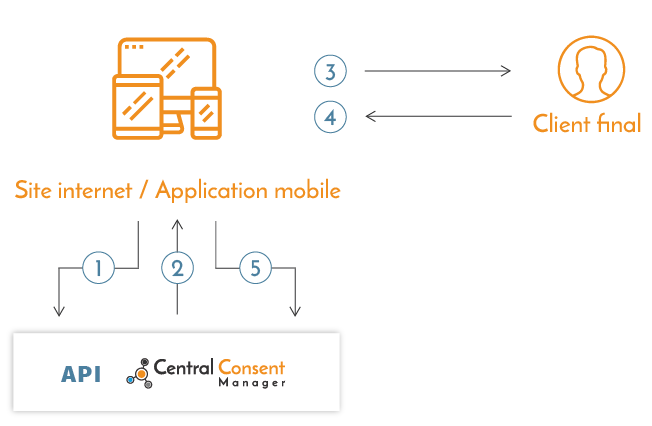
\includegraphics[width=0.8\textwidth]{ccm5.png}
    \end{center}
    \caption{Fonctionnement simplifié de l'application CCM}
\end{figure}
Ci-dessus est schématisé le processus d’enregistrement d’un consentement au sein de la plateforme CCM.
\begin{enumerate}
    \item Requête sur le service de mentions pour un traitement
    \item Envoi des mentions d'informations
    \item Demande de consentement (sous forme d'e-mail ou autre)
    \item Confirmation
    \item Enregistrement du consentement
\end{enumerate}

\section{L’Environnement de travail (culture, évènements d’entreprise...)}
\tab{}Versusmind s’applique à créer une culture d’entreprise autour des valeurs d’échange, du partage,
d’entraide et de la curiosité. La « Versusfamily » communique fréquemment en ligne sur plusieurs
applications : lumapps, par mails, et sur Microsoft Teams.\newline

Les consultants ont la possibilité de publier et de présenter des guides et conseils techniques sur des
nouvelles technologies au travers de conférences mensuelles appelées Symposium (accessibles en
ligne sous forme de vidéo), de témoignages vidéo \#PowerUp d’employés sur différents postes
(disponibles sur la chaine youtube de Versusmind) et d’articles techniques sur le blog « Les Billets de
Versusmind ». Les développeurs peuvent aussi participer à des évènements moins formels mais
toujours techniques comme des Afterwork ou des Hackatons internes d’un weekend, environs tous les
six mois.\newline

En plus de cela, l’agence strasbourgeoise de Versusmind s’applique à rendre les relations entre
collègues conviviales via des activités de team building. Comme un évènement Coding Dojo après le
travail, consistant en la résolution d’un problème ludique en équipe proposée par un maitre de séance.
Dans cette même direction, ludique et amicale, les consultants peuvent se retrouver régulièrement au
sein de soirées jeux de société ou plus généralement « soirées Versusmind » dans les locaux même de
l’agence. Enfin, une fois par mois sont organisés des Bretzmiam, un repas invitant tous les employés
même ceux qui sont mobilisés chez des clients.\newline

Cet environnement de travail a eu beaucoup de poids lorsqu’il m’a fallut choisir mon stage de fin d'études.
\chapter{Développement}
\section{Contexte}
\tab{} Adopté par l’Union Européenne en avril 2016, la date d’entrée en vigueur du RGPD est le 25 mai 2018. Celui-ci oblige les entreprises à identifier les données personnelles en leur possession ainsi que leurs modalités de traitement et de protection et a pour objectifs de\@:
\begin{enumerate}
    \item Uniformiser la réglementation au niveau européen
    \item Responsabiliser les entreprises
    \item Renforcer les droits des personnes
\end{enumerate}
\tab{} Le non-respect du RGPD peut mener à des sanctions financières importantes ainsi qu'a des sanctions administratives ayant un fort impact sur le fonctionnement de l'entreprise.
Il est donc important pour les entreprises d'être en conformité avec le RGPD.\newline
Mais migrer son système d'information pouvant coûter cher, Versusmind propose une solution nommée Central Consent Manager.

\tab{} CCM est système de gestion des consentements centralisé. Il va permettre aux entreprises de se libérer d'un poids en s'assurant que ses utilisateurs ont bien consentis à l'utilisation de leurs données personnelles en centralisant l'enregistrement et la vérification d'authenticité des consentements.

Dans une équipe de développeurs qui évolue beaucoup, mon rôle a été d'aider au développement de la plateforme CCM, à sa mise en production et à améliorer ses performances.
\begin{figure}[H]
    \begin{center}
        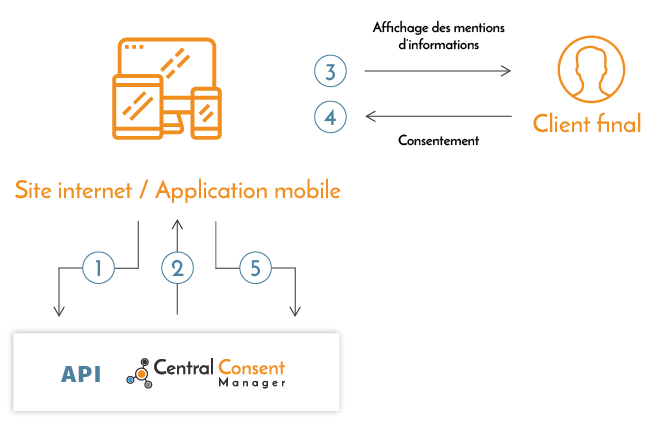
\includegraphics[width=0.8\textwidth]{ccm.png}
    \end{center}
    \caption{Fonctionnement simplifié de l'application CCM}
\end{figure}
\begin{enumerate}
    \item Requête sur le service de mentions pour un traitement
    \item Envoi des mentions d'informations
    \item Demande de consentement (sous forme d'e-mail ou autre)
    \item Confirmation
    \item Enregistrement du consentement
\end{enumerate}
\section{Méthodologie Scrum}
J'ai été intégré durant mon stage à une équipe utilisant la méthodologie Scrum, qui fait partie des méthodes de gestion de projet agiles. Cela vise à supprimer ou au moins à réduire l'effet tunnel d'une méthode de gestion classique par exemple le Cycle en V.\newline
Le développement est découpé en cycles (de trois semaines dans le cas présent) que l'on appelle ``Sprint``.\newline
Les Sprints sont regroupés en saisons afin de représenter un objectif général.
Par exemple, quand j'ai démarré mon stage, le but de la saison en cours était de terminer la refonte graphique.
Au lieu d'un cahier des charges donné au début du projet, on va le découper en User Stories tout au long du projet avec l'aide du client.\newline
Cela permet de rester concentré sur les aspects importants et de ne pas développer de fonctionnalités qui ne seront jamais utilisées.\newline
Un Scrum Master est assigné au projet, son rôle est d'aider l'équipe à bien suivre un fonctionnement agile ainsi qu'a s'organiser. Il est aussi là pour guider le client dans la rédaction des User Stories.
\begin{figure}[H]
    \begin{center}
        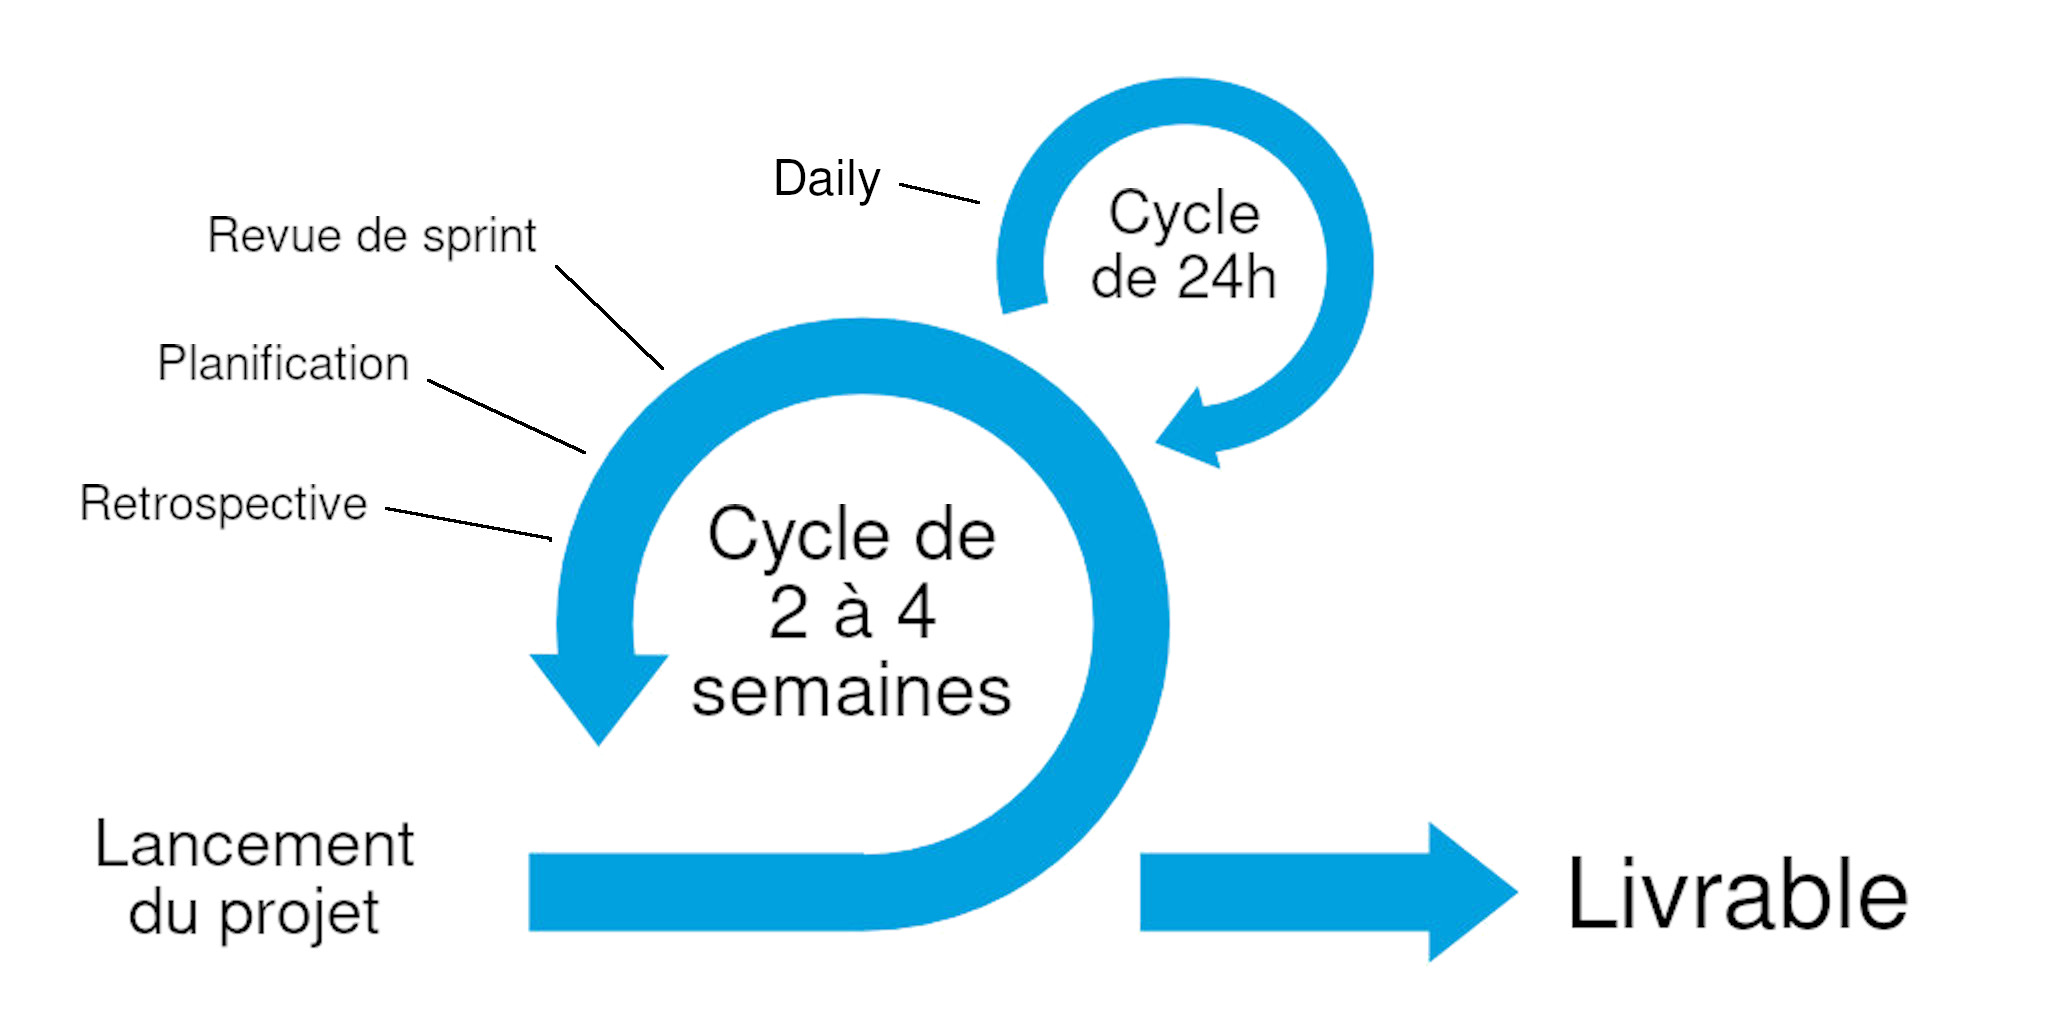
\includegraphics[width=0.9\textwidth]{scrum.jpg}
    \end{center}
    \caption{Cycle de développement Scrum}
\end{figure}
\subsection{Réunions journalières (Daily)}
Chaque matin nous avons une petite réunion qui ne doit pas dépasser 15min afin d'informer rapidement le reste de l'équipe de l'avancement des différentes taches, de discuter brièvement des différents problèmes rencontrés mais aussi de choisir ensemble la priorité des différentes taches qu'il reste à faire.\newline
Cela permet de toujours rester conscient de l'état du projet et d'avoir une vision d'ensemble du travail accompli et du travail restant.
\subsection{Réunions inter-Sprints}
Entre chaque Sprint, une série de réunions nous permet de rester dans la bonne direction concernant le développement du projet.
\subsubsection{Revue de Sprint}
Le but de la revue de Sprint est de montrer à toutes les parties prenantes (Project Owner, Scrum Master, développeurs) l'avancement du projet pendant le dernier Sprint.\newline
L'équipe de développeurs décrit le travail accompli et après une démonstration du résultat, on discute afin de peut-être corriger la direction à prendre pour le prochain Sprint.
\subsubsection{Planification}
S'en suit la planification, elle se fait avec le Scrum Master ainsi que les développeurs.\newline
On va y sélectionner les User Stories à implémenter durant le prochain Sprint. Cela constituera ce qu'on appelle ``L'objectif de Sprint``.\newline
Sous forme d'un nombre on va se mettre d'accord sur une complexité pour chaque User Stories. Cela permet de vérifier qu'on en à bien la même compréhension. Si je propose 1 (facile) et qu'un de mes collègue propose 4 (moyen), c'est que l'un de nous deux à mal compris ce qui est attendu.\newline
Ensuite on découpe chaque User Stories en taches concrètes et enfin on estime le temps de travail sur chaque taches.
\subsubsection{Rétrospective}
Et enfin, encore une fois avec le Scrum Master ainsi que les développeurs, on discute de comment s'est déroulé le dernier Sprint, des pratiques qu'on pourrait mettre en place ou améliorer, mais aussi de comment on l'a vécu et ressenti.\newline
Cela s'inscrit dans un objectif d'amélioration de l'environnement de travail et de l'efficacité.
\section{Architecture}
\begin{figure}[H]
    \begin{center}
        \begin{tikzpicture}
            % nodes
            \node (api) at (1, 1.8) {
\includegraphics[width=0.1\textwidth]{website.png}};
            \node [above=0 of api] {API};
            \node (front) at (1, -1.8) {\begin{overpic}[width=0.1\textwidth]{website.png}
                \put(60, -30){
\includegraphics[scale=.08]{ccm_logo.png}}
            \end{overpic}};
            \node [above=0 of front] {Front-end};
            \node (back) at (6, 0) {
\includegraphics[width=0.1\textwidth]{server.png}};
            \node [above=0 of back] {Back-end};
            \node (function) at (12, 1.8) {
\includegraphics[width=0.1\textwidth]{cloud.png}};
            \node [above=0 of function] {Azure Function};
            \node (ejbca) at (12, -2) {
\includegraphics[width=0.2\textwidth]{ejbca.png}};

            % arrows
            \draw[ultra thick, ->,>=stealth] (api) -- (back);
            \draw[ultra thick, ->,>=stealth] (front) -- (back);
            \draw[ultra thick, double, <->,>=stealth] (back) -- node[above, sloped] {Service Bus} (function);
            \draw[ultra thick, ->,>=stealth] (function) -- (ejbca);

        \end{tikzpicture}
    \end{center}
    \caption{Architecture globale simplifiée}
\end{figure}
Voici un rapide résumé des personnes destinées à utiliser l'application:
\begin{itemize}
    \item Un administrateur Versusmind, qui pourra, via le Back-Office, accéder aux contrats souscrits avec les entreprises. Il n'a pas besoin de compétences techniques.
    \item Un administrateurs client, qui pourra, via le Back-Office, ajouter des traitements et des consentements. Il n'a pas besoin d'avoir de compétences techniques.
    \item Les développeurs clients, qui accédent à l'API du Back-end afin d'intégrer CCM dans leurs solution déjà existante.
    \item Les utilisateurs finaux, qui donneront leurs consentements au travers de la plateforme.
\end{itemize}
Tout d'abords je vais rapidement expliquer l'architecture du projet.
La solution CCM est composée de différents éléments:
\begin{itemize}
    \item Une partie Font-end écrite en HTML/CSS/Typescript avec le framework Angular, c'est le back-office d'administration, il sert les différentes pages web à l'utilisateur.
    \item Une partie Back-end écrite en Java avec le framework Spring Boot, c'est le cœur de l'application, elle peut recevoir des requêtes via le Front-end ou directement par API
    \item La gestion du chiffrement est en deux parties
        \begin{itemize}
            \item Une instance EBJCA qui prends le rôle d'autorité de certification
            \item Des Fonctions Azure écritent en Java qui chiffrent et vérifient les consentements. Elles communiquent avec le Back-end via des Service Bus Azure (de simples files d'attentes de messages JSON)
        \end{itemize}
    \item Une instance Redis afin de garder du cache des différentes requêtes faites à la base de données.
\end{itemize}
\subsection{Outils}
\tab{}Les différentes parties du stystème sont hébergées sur plateforme cloud Microsoft Azure.\newline
On utilise aussi Azure DevOps afin d'informatiser les notions de Sprints et de User Stories mais aussi pour faciliter la gestion du code source, jouer les jeux de tests et automatiser le déploiement des nouvelles versions.\newline

\tab{}Concernant mon poste de travail, j'ai eu l'agréable surprise de pouvoir travailler avec l'environnement de mon choix et l'IDE ou éditeur de texte de mon choix. J'ai donc pu installer la distribution Arch Linux ainsi que mes configurations habituelles et cela a grandement participé au confort au quotidien. J'ai développé en utilisant NeoVim (qui est une réécriture de l'éditeur Vim) couplé à un ensemble de modules et notamment le module Conquer of Completion (Coc) qui permet d'utiliser de multiples serveurs de languages dérivés des implémentations utilisées par Visual Studio Code. J'ai donc pu profiter d'une autocomplétion intélligente identique à celle de mes collègues de travail qui utilisent Visual Studio Code.
\subsection{Front-end}
\subsubsection{Angular}
\tab{}J'ai commencé mon stage en me formant sur l'utilisation du framework Angular sur lequel je suis maintenant à l'aise.\newline
Angular est un framework front-end destiné à faciliter la création de pages web en utilisant le patern model-vue-controlleur.

L'interface web se découpe en une multitude de composants imbriqués les uns dans les autres.
Ces composants utilisent des services afin commiquer avec le back-end, et affichent des données à l'écran au travers de templates HTML.
La mise en place d'un nouveau composant nécessite de définir un certain nombre d'éléments:
\begin{itemize}
    \item Les données dont le composants à besoin. Ses entrées
    \item Les événements produits par le composant. Ses sorties
    \item Les différents services et autres composants dont dépend le composant. Ses dépendances
    \item Sont design visuel. Son template\newline
\end{itemize}
Mais certaines parties sont plus spécifiques. Comme par exemple la gestion des traductions et la gestion de l'authentification.
Dans notre projet il existe deux fichiers JSON associants des clés de traductions à des valeurs. Chacun des fichiers comportants les traductions d'une langue précise, par exemple:\newline
En anglais:
\begin{lstlisting}
{
    "pageTitle": "Consents"
}
\end{lstlisting}
En Francais:
\begin{lstlisting}
{
    "pageTitle": "Consentements"
}
\end{lstlisting}
Et nous pourrons utiliser la clé \textbf{pageTitle} afin d'automatiquement afficher la bonne traduction en fonction de la langue choisie.\newline

Concernant l'authentification, il s'agit d'un service qui va écouter l'ensemble des retours HTTP faits au back-end, et si l'un d'entre eux retourne un code d'erreu 401 (signifiant que l'utilisateur n'est pas authentifié), le service s'occupera d'enregistrer la page courante, de rediriger l'utilisateur sur la page d'authentification pour enfin le faire revenir sur la page ou il était.\newline

J'ai pu ensuite aider à la fermeture d'une saison de refonte graphique en apportant mes connaissances et mon expérience en intégration web à l'équipe.\newline
J'ai aussi participé à l'amélioration et à l'enrichissement de l'interface sur toute le reste de mon stage. En modifiant des composants que ce soit pour fixer un comportement non voulu ou pour ajouter des fonctionnalités. Mais aussi en ajoutant de nouveaux composants avec l'aide de l'équipe UX, chargée de livrer des maquettes de designs d'interfaces et d'expérience utilisateur.\newline
\subsubsection{CSS}
\tab{}Tout au long de ma formation, j'ai pu faire de la veille technologique et guider l'équipe vers une restructuration de l'architecture CSS plus maintenable et plus facile à étendre.\newline
Cela se concrétise par la rédaction d'un guide de bonne pratiques que les développeurs peuvent consulter lors de la modification, l'extension ou la création d'un composant graphique.
Afin de rédiger ce guide, j'ai du aussi me baser sur l'architecture existante afin de ne pas viser un but parfait mais inatteignable à cause de la dette technique actuelle.\newline
J'aborde dans ce guide, la notion de précision en CSS afin d'aider les développeurs à mieux comprendre les conflits qu'ils peuvent rencontrer et d'éviter l'utilisation abusive de la directive "!important". Je propose d'utiliser la convention de nommage BEM, afin de mieux gèrer la précision et la modulatiré de nos règles CSS. J'apporte aussi quelques notes sur l'utilisation de préprocesseurs CSS et de dépendances externes tels que Angular Matérial dans notre cas.\newline
La rédaction m'a été confiée suite à de multiples phases de relecture de code à plusieurs ou mes collègues se sont apercu que j'appréciais le développement de mise en page web. Après plusieurs jours de rédaction, mise au points je l'ai soumis à mes collègues le 13 Janvier, il a pu être relu et discuté par l'équipe et après quelques clarifications à été validé dans la journée.\newline
\begin{figure}[H]
    \begin{center}
        \fbox{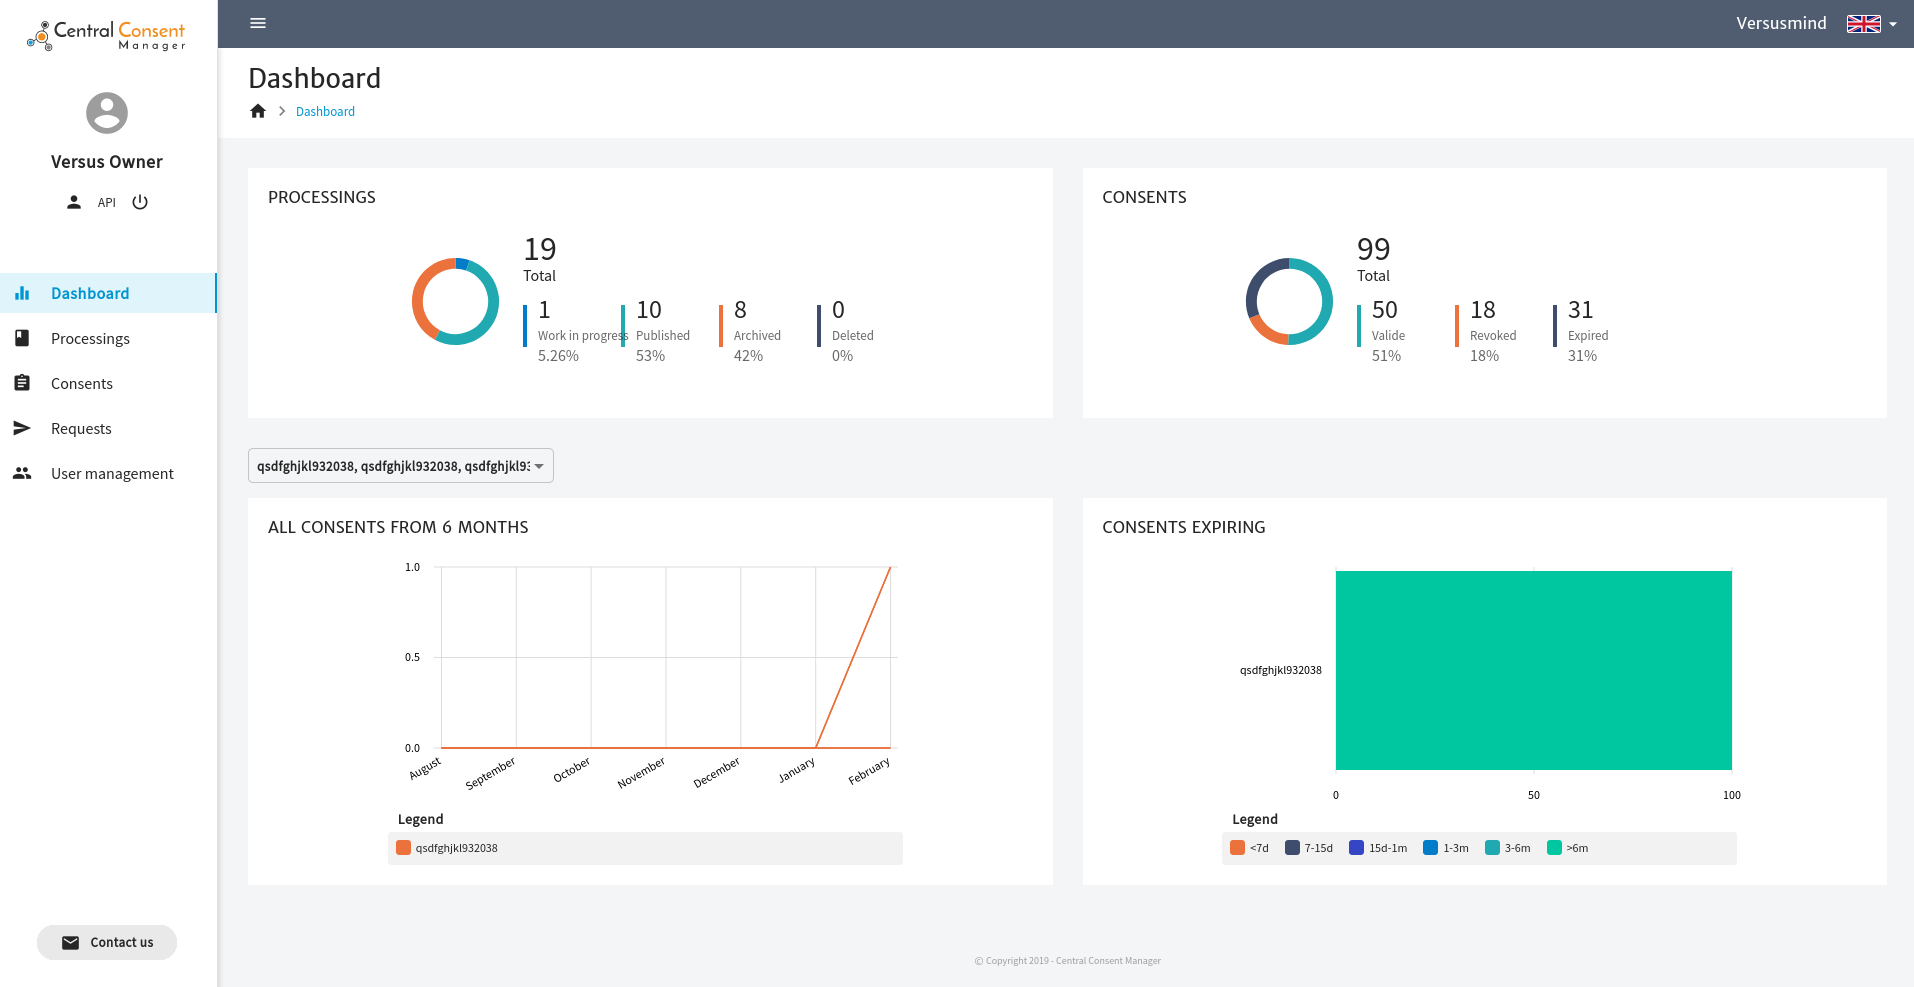
\includegraphics[width=\linewidth]{ccm_dashboard.png}}
    \end{center}
    \caption{Page d'accueil de l'application}
\end{figure}
\begin{figure}[H]
    \begin{center}
        \fbox{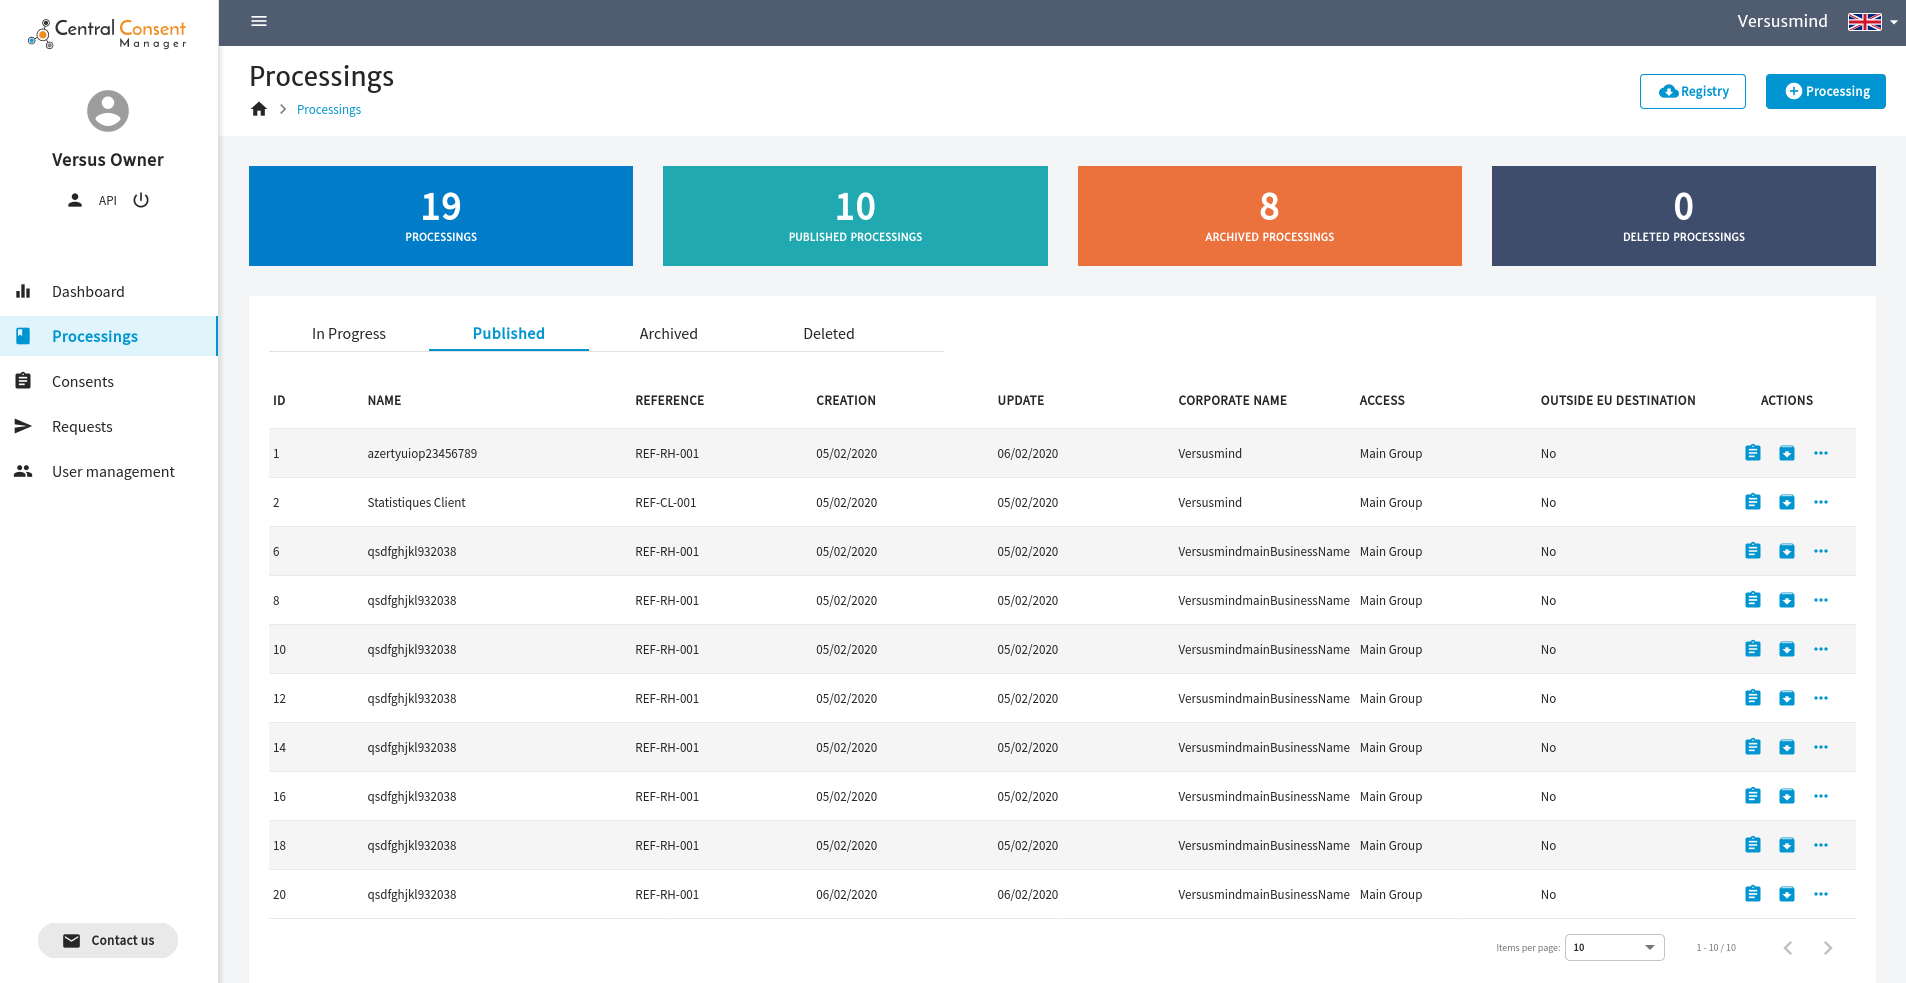
\includegraphics[width=\linewidth]{ccm_processing_list.png}}
    \end{center}
    \caption{Liste des traitements}
\end{figure}
\begin{figure}[H]
    \begin{center}
        \fbox{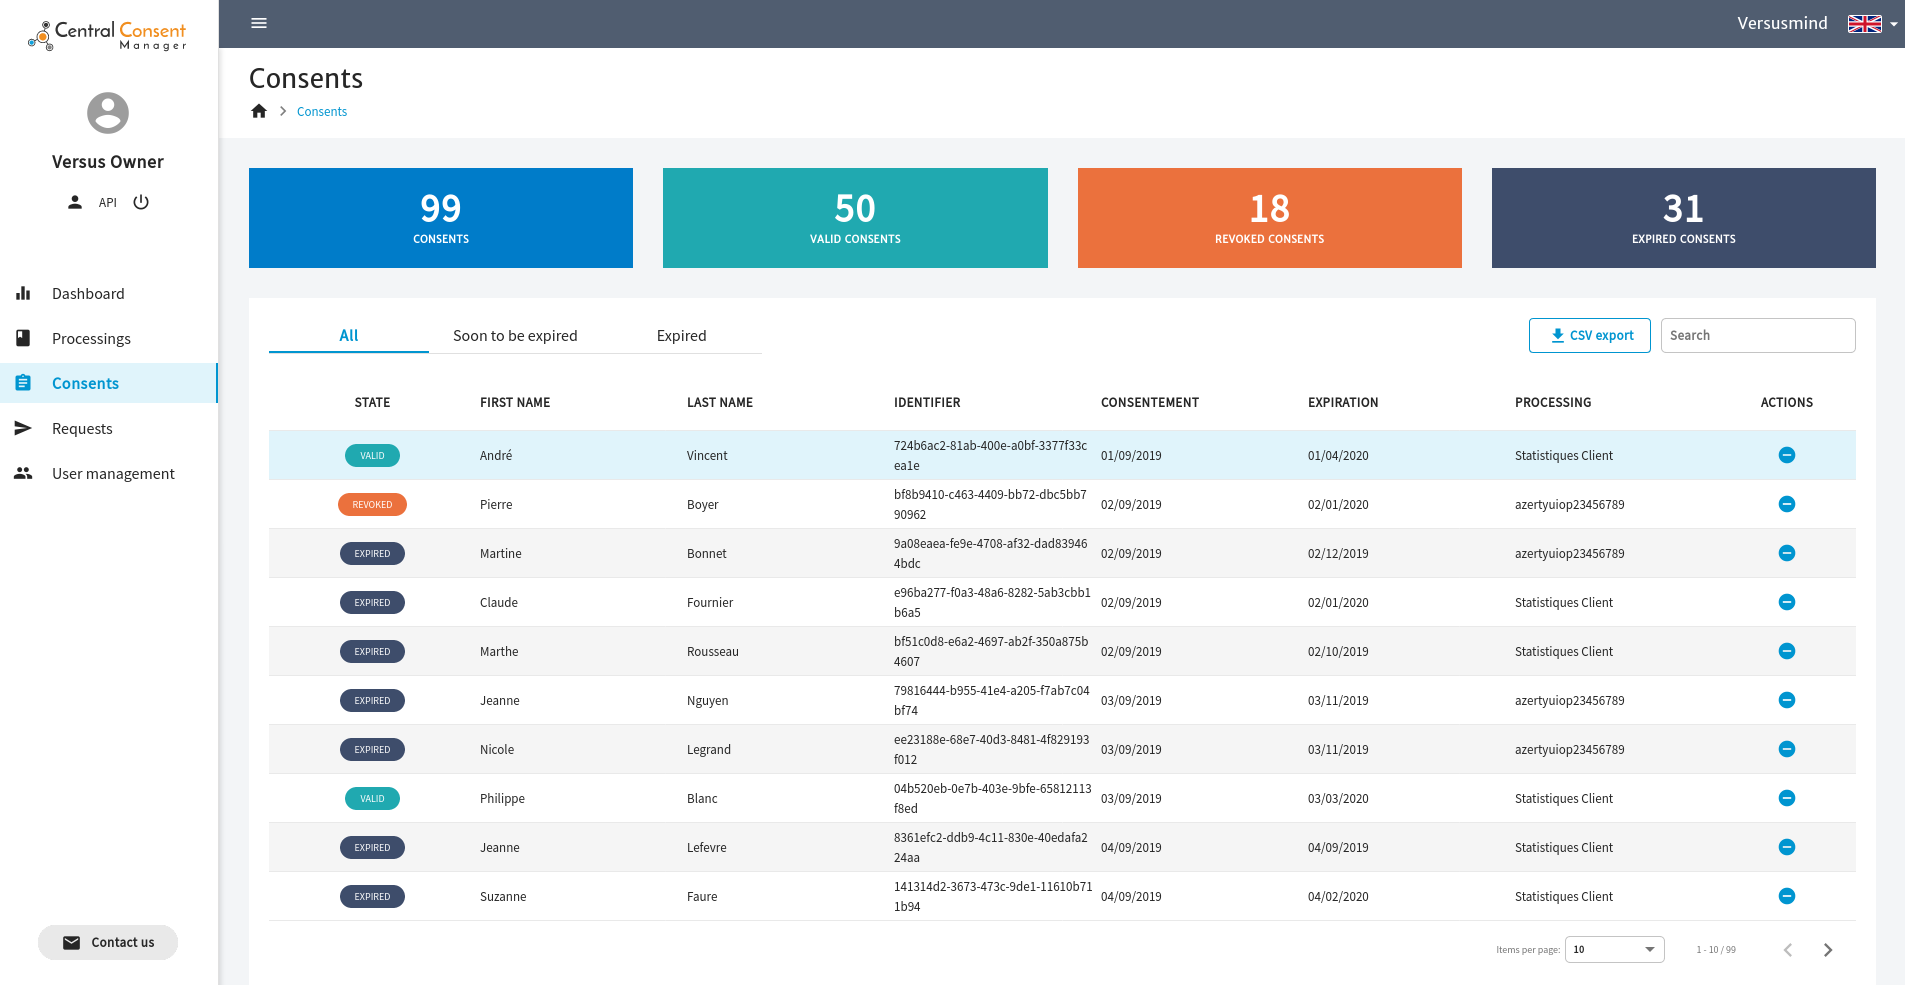
\includegraphics[width=\linewidth]{ccm_consentement_list.png}}
    \end{center}
    \caption{Liste des consentements}
\end{figure}
\begin{figure}[H]
    \begin{center}
        \fbox{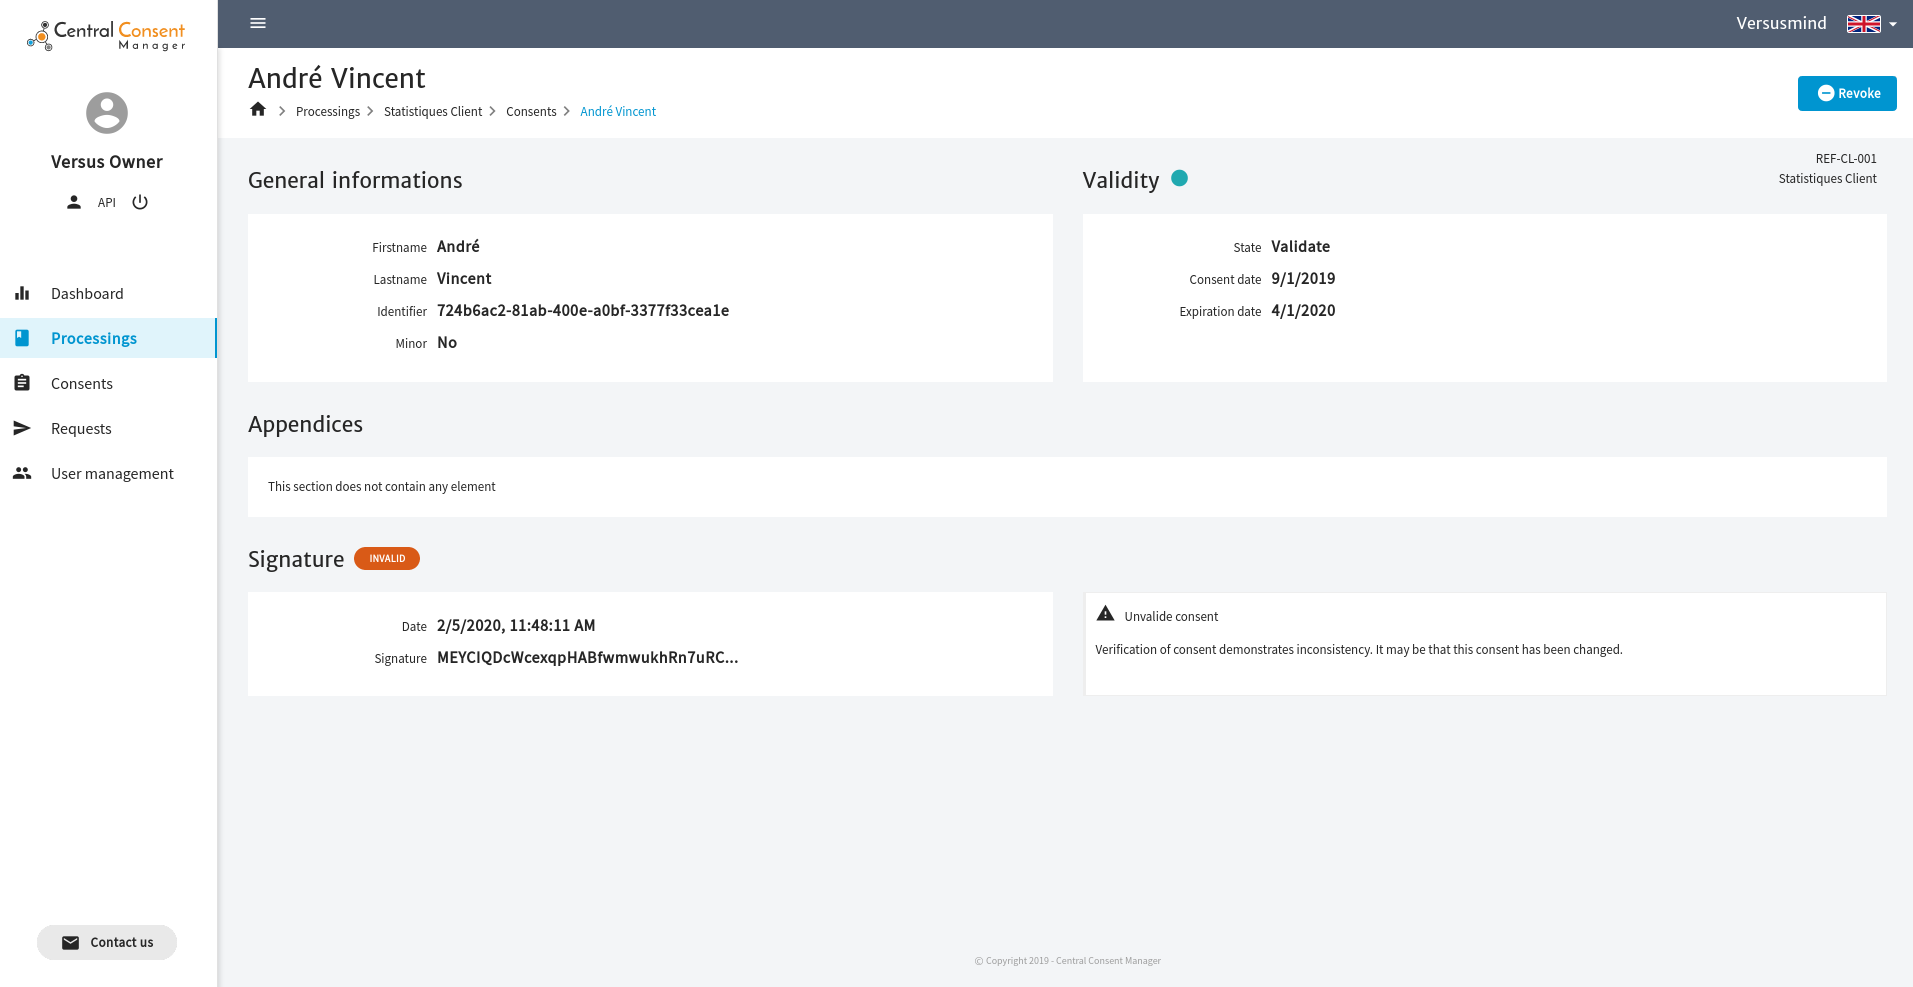
\includegraphics[width=\linewidth]{ccm_consentement_detail.png}}
    \end{center}
    \caption{Détail d'un consentement}
\end{figure}
\newpage
\subsection{Back-end}
Le back-end est développé à l'aide de Spring, un framework open source permettant la création simple d'infrastructure Java simple et facilement testable.\newline

L'application est divisée en trois niveaux,\newline
Les contrôleurs qui vont recevoir les requêtes HTTP, que ce soit via une intégration de l'API sur le site d'un client, ou du backoffice de CCM. Leur rôle est de correctement mettre en forme et rediriger les données aux bons services.\newline
C'est ensuite la responsabilité de la couche Business de vérifier les droits d'accès, l'intégrité des données et enfin de demander une mise à jour ou une récupération en base de données.\newline
Cette dernière est gérée par la couche Repository qui va, au travers de requêtes générées par l'ORM ou de requêtes SQL forgées manuellement, communiquer avec la base de données.\newline

J'ai contribué au développement du back-end du projet, sous forme d'ajout de fonctionnalités, correction de failles de sécurité, correction de bugs, etc\ldots
\subsubsection{Gestion du cache}
Je n'ai pas touché au développement de la gestion du cache côté serveur, mais j'ai participé aux discussions et aidé à la prise de décisions.
Nous avons fait face à un problème de mise à jour des données présentes à la fois dans la base de données et dans le cache. La solution vers laquelle nous nous sommes orientés est de simplifier les requêtes faites en base pour unifier la récupération des données (abstraire le cache et la base de données) et de filtrer les données dans une couche applicative.
\subsection{Certification numérique}
J'ai eu à déployer une instance EJBCA assignée à l'instance de production de la plateforme CCM.\newline
EJBCA ou Enterprise JavaBeans Certificate Authority est une solution d'autorité de certification libre et open source proposée par PrimeKey.

Mon travail dans cette tache s'est étendu de la génération de clés cryptographiques, à la manipulation de la plateforme Azure et du stockage de mots de passe sensibles car liés à la production.
\subsection{Montée en charge}
\tab{} Suite à la refonte graphique, nous sommes entrés dans une saison de mise en production et deux problématiques de performances sont apparues assez vite:
\begin{itemize}
    \item Lorsqu'un nouveau client veux migrer vers CCM, une base de consentements potentiellement conséquente doit être importée.
    \item Un client doit pouvoir exporter cette base sous forme de fichier, ce qui implique une vérification de validité d'un grand nombre de consentements.
\end{itemize}

Suite à des tests de charge, nous avons observé qu'il faudrait environ 3 jours pour importer une base d'un million de consentements. Et plusieurs heures pour générer un export des consentements enregistrés. Ce n'était pas acceptable.\newpage
\subsubsection{Signature}
J'ai eu la responsabilité d'implémenter les fonctions Azure afin de paralléliser chaque création de signature numérique.
\begin{figure}[H]
    \begin{center}
        \begin{tikzpicture}
            % nodes
            \node (consentement) at (-6, 0) {
\includegraphics[width=0.1\textwidth]{file.png}};
            \node [above=0 of consentement] {Consentement};
            \node (function) at (0, 0) {
\includegraphics[width=0.1\textwidth]{cloud.png}};
            \node [above=0 of function] {Azure Function};
            \node (ejbca) at (0, -3) {
\includegraphics[width=0.2\textwidth]{ejbca.png}};
            \node (consentement2) at (6, 0) {\begin{overpic}[width=0.1\textwidth]{file.png}
                \put(60, -20){
\includegraphics[scale=.05]{lock.png}}
            \end{overpic}};
            \node [above=0 of consentement2] {Consentement signé};

            % arrows
            \draw[ultra thick, ->,>=stealth] (consentement) -- (function);
            \draw[ultra thick, ->,>=stealth] (function) -- node[left] {
\includegraphics[width=0.06\textwidth]{key.png}} (ejbca);
            \draw[ultra thick, ->,>=stealth] (function) -- (consentement2);

        \end{tikzpicture}
    \end{center}
    \caption{Parcours de la signature d'un consentement}
\end{figure}
Dans la même tâche, j'ai pu implémenter la révocation de consentement en utilisant aussi des fonctions Azure.
\subsubsection{Vérification}
J'ai aussi eu à travailler sur la vérification des consentements et j'ai pu diviser le temps de signature par 2 tout en augmentant drastiquement le niveau de sécurité.
\begin{figure}[H]
    \begin{center}
        \begin{tikzpicture}
            % nodes
            \node (consentement) at (-6, 0) {\begin{overpic}[width=0.1\textwidth]{file.png}
                \put(60, -20){
\includegraphics[scale=.05]{lock.png}}
            \end{overpic}};
            \node [above=0 of consentement] {Consentement signé};
            \node (server) at (0, 0) {
\includegraphics[width=0.1\textwidth]{server.png}};
            \node [above=0 of server] {Back-end (multithread)};
            \node (ejbca) at (0, -3) {
\includegraphics[width=0.2\textwidth]{ejbca.png}};
            \node (verified) at (7, 0) {
\includegraphics[width=0.1\textwidth]{verified.png}};
            \node [above=0 of verified] {Validé};

            % arrows
            \draw[ultra thick, ->,>=stealth] (consentement) -- (server);
            \draw[ultra thick, ->,>=stealth] (ejbca) -- node[right] {
\includegraphics[width=0.06\textwidth]{key.png}} (function);
            \draw[ultra thick, ->,>=stealth] (server) -- (verified);

        \end{tikzpicture}
    \end{center}
    \caption{Parcours de vérification d'un consentement non altéré}
\end{figure}
\begin{figure}[H]
    \begin{center}
        \begin{tikzpicture}
            % nodes
            \node (ejbca) at (0, -3) {
\includegraphics[width=0.2\textwidth]{ejbca.png}};
            \node (consentement2) at (-6, 0) {\begin{overpic}[width=0.1\textwidth]{file.png}
                \put(60, -20){
\includegraphics[scale=.05]{lock2.png}}
            \end{overpic}};
            \node [above=0 of consentement2] {Consentement altéré};
            \node (server2) at (0, 0) {
\includegraphics[width=0.1\textwidth]{server.png}};
            \node [above=0 of server2] {Back-end (multithread)};
            \node (error) at (6, 0) {
\includegraphics[width=0.1\textwidth]{error.png}};
            \node [above=0 of error] {Données corrompues};

            % arrows
            \draw[ultra thick, ->,>=stealth] (consentement2) -- (server2);
            \draw[ultra thick, ->,>=stealth] (ejbca) -- node[right] {
\includegraphics[width=0.06\textwidth]{key.png}} (server2);
            \draw[ultra thick, ->,>=stealth] (server2) -- (error);

        \end{tikzpicture}
    \end{center}
    \caption{Parcours de vérification d'un consentement altéré}
\end{figure}
\section{Développement dirigé par les tests (TDD)}
Durant mon stage, j'ai appris à implémenter des tests afin de subvenir à plusieurs besoins\@:
\begin{enumerate}
    \item Fournir une preuve de fonctionnement du code testé
    \item Prévenir d'éventuels bugs futurs
    \item S'assurer du bon fonctionnement de l'application avant son déploiement
\end{enumerate}
Le développement suit un cycle circulaire ou nous développons des nouvelles fonctionnalités, ce qui change le comportement de l'application, les tests ne passent donc plus. Nous réparons les test, et le cycle recommence.
\begin{figure}[H]
    \begin{center}
        \includegraphics[width=0.5\linewidth]{TDD.jpg}
    \end{center}
    \caption{Cycle de tests et de développement}
\end{figure}
Pour cela, on défini le comportement unitaire de chaque composant, ainsi qu'un ou plusieurs parcours d'utilisation critiques utilisant les éléments clés de l'application.\newline
J'ai eu l'occasion de créer différents types de tests\@:
\begin{description}
    \item [Les tests unitaires] s'assurent que chaque composant de l'application rempli son rôle.
    \item [Les tests d'intégrations] vérifient un fonctionnement comportant plusieurs composants.
    \item [Les test de bout en bout] implémentent des User Stories completes, utilisant toutes les couches de l'application.
\end{description}
Et dans une démarche d'intégration continue j'ai participé à la mise en place de systèmes de tests et de déploiement automatisés sur la plateforme Azure DevOps.\newline
J'ai pu utiliser les solutions SonarQube pour le Back-end et Eslint pour le Front-end qui s'occupent d'analyser le dépôt de code source afin d'y trouver des problèmes de sécurité, des bugs, des mauvaises pratiques ainsi que de la duplication de code.\newline
Cela contribue à rendre le code plus stable et plus maintenable.\newline
\chapter{Conclusion}
Ce stage m'a beaucoup apporté, d'un point de vue technique mais aussi au niveau organisationnel.\newline
C'est pour moi une première expérience professionnelle suivant une méthode agile et j'en suis satisfait.
Les réunions régulières m'ont permises de prendre du recul sur le travail effectué, et le travail en équipe agile à créé une dynamique dans laquelle nous nous poussions mutuellement vers le haut.\newline
J'y ai appris à suivre un processus de développement plus stable, grâce au développement dirigé par les tests ainsi qu'a l'intégration continue via Azure DevOps.\newline
J'ai aussi appris à développer des tests de charge et à interpréter leurs résultats afin d'en tirer des directions à prendre.\newline
En définitive, même si le développement web n'est pas mon domaine favori, j'ai vécu une belle expérience durant ce stage et j'ai la chance de pouvoir rester au près de Versusmind et de peut-être approfondir des sujets qui me tiennent plus à cœur.
\appendix
\chapter{Personas}
Les différents rôles dans l'application:
\subsubsection{Versusmind}
La société éditrice du logiciel
\subsubsection{Propriétaire}
La personne physique représentant le Responsable de traitement (Directeur général/Président par exemple) et ayant la capacité d'engager l'organisme.
\subsubsection{Admin client}
Par exemple: Un RSSI et/ou un Délégué à la protection des données (DPO) qui doivent pouvoir avoir tous les droits de lecture/écriture ainsi qu'un droit de gestion des Utilisateurs / Consultant.\newline
Le RSSI et le DPO gèrent conjointement le projet de mise en conformité au RGPD au sein d'un organisme.\newline
Si aucun des deux acteurs n'est nommé au sein d'un organisme et n'a pas vocation à être nommé, il est recommandé de désigner un "Référent données personnelles" ayant en charge le projet de mise en conformité.
\newpage
\subsubsection{Utilisateurs}
Par exemple : Le directeur/directrice du service communication de l'organisme qui souhaite créer une newsletter en lien avec les clients de l'organisme ou des prospects ayant consenti sur le site internet de l'organisme.\newline
Cette newsletter nécessite le consentement des clients et doit apparaître au registre des traitements.\newline
Le directeur/directrice du service communication complète donc la partie correspondante dans le registre après que le RSSI et/ou le DPO ou, à défaut, le "Référent données personnelles" lui a octroyé les droits.
\subsubsection{Consultant}
Un consultant est une personne qui n'a que des droits de lecture sur le registre ou le consentement.\newline
Par exemple: Une personne du service communication qui doit suivre les consentement sans avoir besoin de les modifier.\newline
Ou encore: Une stagiaire qui a besoin d'y accéder pour travailler mais n'a pas soit la responsabilité nécessaire, soit le besoin de bénéficier d'un droit d'écriture.\newline
\chapter{Guide CSS}
\subsection{Et si ca devenait agréable de faire du CSS ?}

Pour beaucoup de développeurs, le CSS a une image d'un langage qu'il faut sans arrêt bricoler pour arriver à nos fins.
Une des raisons principales est que le CSS est très permissif et ne propose pas d'architecture en lui-même, c'est un grand bac a sable.
En conséquences, si un projet grossi, la structure CSS choisie (ou construite de manière empirique) finie par être un cauchemar à maintenir et à étendre tant il y a de collisions de règles.
Un indicateur d'un projet ayant grossi sans avoir fait évoluer sa structure CSS est le nombre de \textbf{!important} dans le code. Cela montre des conflits n'ayant pas été résolus, mais masqués (Je reviendrais sur ce point).

Je vais donc ici vous proposer une architecture CSS qui va vous permettre d'organiser votre code, de le documenter, d'éviter les conflits mais aussi d'améliorer la maintenabilité et faciliter l'extension.

Rapidement pour que tout le monde soit d'accord sur les termes que j'utilise:
\begin{lstlisting}
    regle {
        propriété: valeur;
        propriété: valeur !important;
    }
\end{lstlisting}

\subsubsection{La précision}

Afin de comprendre et d'éviter les conflits dans le code, il faut se préoccuper de la notion de 'précision' d'une règle CSS.
Si il y a conflit sur une propriété, c'est la règle avec la plus grande précision qui l'emporte, sauf si il y a la directive \textbf{!important}.
Si deux propriétés sont en conflit avec la même précision, c'est la règle déclarée en dernier qui l'emporte (l'ordre a son importance !).

La précision d'une règle augmente avec le nombre de membres qu'elle contient.
\begin{lstlisting}
body { // précision: 1
[...]
}

body p { // précision: 2
[...]
}

body > p { // précision: 2
[...]
}

.container { // précision: 1
[...]
}

.container.disabled { // précision: 2
[...]
}
\end{lstlisting}

Attention à l'utilisation de préprocesseurs CSS, toujours penser à la précision des règles qui seront génerées:
\begin{lstlisting}
body {
    [...]

    p {
        [...]

        &.selected {
            [...]
        }
    }
}
\end{lstlisting}
Compilera en:
\begin{lstlisting}
    body { // précision: 1
    [...]
    }

    body p { // précision: 2
    [...]
    }

    body p.selected { // précision: 3
    [...]
    }
\end{lstlisting}

La précision d'une règle contenant un identifiant est infinie, elle écrasera n'importe quelle propriété lors d'un conflit.
Cela rend l'extension du code impossible, c'est donc à proscrire dans vos bases de code CSS.

\begin{lstlisting}
    #page { // précision infinie
    [...]
    }
\end{lstlisting}

De manière générale, il faut essayer de toujours garder la précision la plus basse possible.


\subsubsection{Structure HTML}

Il arrive régulierement que lors de corrections ou d'extensions des fonctionnalités, qu'il faille changer la structure HTML d'une page.
Si les règles CSS se basent exclusivement sur cette dernière, les propriétés ne cibleront peut-être plus les bons blocs HTML.
Cela implique plus de maintenance et de la résilience à l'extension.
Il faut donc éviter au maximum de se baser sur la structure HTML afin de définir du style.
De manière générale il ne faut pas définir un élément en fonction de où il est, mais ce qu'il est.
Il faut donc préférer définir des classes spécifiques qui concernent le cas d'application précis de l'élément.

\begin{lstlisting}
    nav button {
        [...]
    }
\end{lstlisting}

Pourrait être:

\begin{lstlisting}
    .button--nav {
        [...]
    }
\end{lstlisting}

Cela réduit la dépendence à la structure HTML et cela a aussi réduit la précision, parfait.

\subsubsection{Découpage en composants + convention de nommage}

Voici un point qui va grandement (et je pèse mes mots) améliorer la facilité de lecture et donc de maintenance de votre code.
C'est la suite logique du point précédent où il va falloir définir des composants et les isoler de leur environnement.
Je vous propose la convention de nommage BEM pour (Bloc, Element, Modifier)
Cela va permettre de standardiser le nommage de vos classes et faciliter la lecture du code.

Prenons l'exemple d'un simple article:
\begin{itemize}
    \item définition de la racine du bloc: \textbf{article}
    \item des éléments qui le composent: \textbf{titre}, \textbf{contenu}
    \item et enfin des spécialisations du bloc: \textbf{informatique}, \textbf{general}
    \item dans son propre fichier du nom du composant: \textbf{\textunderscore article.scss}
\end{itemize}

\begin{lstlisting}
    .article {
        [...]
    }

    .article--menuiserie {
        [...]
    }

    .article--informatique {
        [...]
    }

    .article__titre {
        [...]
    }

    .article__contenu {
        [...]
    }
\end{lstlisting}

La même chose avec Sass:

\begin{lstlisting}
    .article {
        [...]

        &--menuiserie {
            [...]
        }

        &--informatique {
            [...]
        }

        &__titre {
            [...]
        }

        &__contenu {
            [...]
        }
    }
\end{lstlisting}

Et appliqué à du HTML:

\begin{lstlisting}
    <body>
    <div class="article article--informatique">
    <div class="article__titre">
    Et si ça devenait agréable de faire du CSS ?
    </div>
    <div class="article__contenu">
    [...]
    </div>
    </div>
    <div class="article article--Menuiserie">
    <div class="article__titre">
    L'utilisation de la scie sauteuse en milieu urbain
    </div>
    <div class="article__contenu">
    [...]
    </div>
    </div>
    </body>
\end{lstlisting}

C'est en effet plus verbeux qu'une méthode moins structurée, mais à grande échelle, cela compartimente correctement les comportements attendus.
Attention toutefois au nommage de vos spécialisations ! Il ne faut pas nommer une spécialisation par une valeur qu'elle comporte, car si cette valeur change, le nom de la classe n'aura plus de sens.
Par exemple, ne pas utiliser \textbf{.article--rouge} mais plutôt spécifier la sémantique, le sens qu'il porte : \textbf{.article--important}.

\subsubsection{!important}

Maintenant que nous avons aborder comment éviter les conflits, pourquoi avoir besoin de la directive \textbf{!important} ? Pourquoi existe-t-elle si nous pouvons nous en passer ?
Simplement car cette directive doit-être utilisée de manière proactive et non réactive.
L'utiliser en réponse à un conflit que difficile à résoudre soulève un problème de précision dans l'architecture.
Par contre, il est possible de l'utiliser dans un cas où l'on sait déjà en amont qu'une propriété DOIT surpasser toute autre règle, par exemple dans le cas d'un plein écran:

\begin{lstlisting}
    .article {
        [...]

        &--fullscreen {
            position: absolute !important;
            width: 100vw !important;
            height: 100vh !important;
        }
    }
\end{lstlisting}

Si ces propriétés ne sont plus désirées, c'est qu'il faut retirer la classe du HTML.

\subsubsection{Les dépendances externes}

Les dépendances externes peuvent parfois avoir des précisions plus grandes que les règles de notre code.
Au lieu de placer la directive \textbf{!important} afin de résoudre le problème et passer à la suite, ou encore de se baser sur la structure du HTML pour augmenter la précision, voici une petite astuce:

\begin{lstlisting}
    .classe-externe.classe-externe { // Précision: 2
    [...]
    }
\end{lstlisting}

Cela augmente la précision de la règle, ce qui est obligatoire si l'on veut changer le comportement du code, mais sans aucune dépendance de classe et sans détruire l'arbre de précision avec un \textbf{!important}.

\subsubsection{Documentation}

Et enfin le meilleur pour la fin, la documentation.
Après avoir refondu toute la structure et appliqué tous ces superbes conseils, il nous manque encore de la documentation afin de se rappeler du comportement d'un bloc, d'un élément ou d'une spécialisation.
Je vous propose une documentation simple en entête de chaque fichier de composant.
Grouper chaque élément et ses spécialisations et séparer les éléments entre eux afin de bien visualiser les différents groupes de règles :

\begin{lstlisting}
// .article
//     Composant représentant un article de blog
// .article--menuiserie
//     Spécialisation d'un article concernant la menuiserie
// .article--informatique
//     Spécialisation d'un article concernant l'informatique
//
// .article__titre
//     Élement titre d'un article
//
// .article__contenu
//     Élement de contenu d'un article
//
// Exemple:
// <div class="article article--informatique">
//     <div class="article__titre">
//         [...]
//     </div>
//     <div class="article__contenu">
//         [...]
//     </div>
// </div>

.article {
    [...]

    &--menuiserie {
        [...]
    }

    &--informatique {
        [...]
    }

    &__titre {
        [...]
    }

    &__contenu {
        [...]
    }
}
\end{lstlisting}

\subsubsection{Conclusion}

Nous y voilà, nous avons vu qu'il faut décrire des composants pour ce qu'ils sont et non pour leur emplacement dans la page.
Nous savons maintenant qu'il ne faut pas utiliser d'identifiant dans le CSS mais aussi qu'il faut utiliser \textbf{!important} avec parcimonie.
Nous avons aussi vu qu'utiliser une convention de nommage en CSS permet d'ajouter du sens dans notre code sans augmenter la précision.
Et enfin nous avons vu comment documenter nos classes CSS pour s'y retrouver et que chaque composant soit indépendant.

Si vous étiez fachés avec le CSS et que vous êtes arrivés jusqu'ici, déjà bravo, et j'espère vous avoir au moins un peu réconcilié avec ce language.
Sinon j'espère vous avoir quand même apporté quelque chose au travers de cet article.

\listoffigures
\makeutbmbackcover{}
\end{document}
